\documentclass[11pt]{article}

\def\articlename{资产定价}
\def\authorname{杨弘毅}
\def\startdate{2021年6月10日}

\ifx \authorname\undefined
  \def\authorname{杨弘毅}
\else
\fi

\author{\authorname}
\date{创建:\startdate \\修改:\today}

\usepackage[a4paper,left=6em,right=6em]{geometry}
\usepackage{amsmath,amsfonts,amsthm,bbold}
\usepackage{booktabs,float,multirow}
\usepackage{cancel}
\usepackage{enumitem}
\usepackage{multicol}
\usepackage{graphicx}
\usepackage[toc,title]{appendix}
\usepackage{tikz}
\usetikzlibrary{arrows.meta}
\usetikzlibrary{patterns}
\usetikzlibrary{decorations.pathreplacing}
\usetikzlibrary{decorations.pathmorphing}
\usepackage{subcaption}
\usepackage{fancyhdr}
\pagestyle{fancy}
\setlength{\headheight}{15pt}
\usepackage{footmisc}
\usepackage{hyperref}
\usepackage{tocloft}
\hypersetup{
    colorlinks=true, %set true if you want colored links
    linkcolor=blue,
    linktoc=all, %set to all if you want both sections and subsections linked
    citecolor=black,
    filecolor=black,
    urlcolor=blue
}
\usepackage[UTF8]{ctex}

\title{\articlename}

% Format
\setlength{\cftbeforesecskip}{6pt}
\setlength{\parskip}{0.6em}
\renewcommand{\baselinestretch}{1.4}
\setlist{noitemsep,itemindent=1em,topsep=0em,leftmargin=4em,rightmargin=4em}
\setlist[2]{leftmargin=2em}

% Shortcut
\newcommand{\divider}{\vspace{-\parskip}\noindent\rule{\linewidth}{0.4pt}}
\newcommand{\tops}[1]{\texorpdfstring{#1}{TEXT}}

% Theorem
\newtheorem{thm}{定理}[section] 
\newtheorem{proposition}[thm]{命题}
\newtheorem{lemma}[thm]{引理}
\newtheorem{corollary}[thm]{推论}
\newtheorem{property}[thm]{性质}
\newtheorem{example}[thm]{例子}
\newtheorem{remark}[thm]{备注}
\newtheorem{note}[thm]{注释}

% Symbol
\newcommand{\E}{\mathbb{E}}
\newcommand{\mcl}{\mathcal{L}}
\newcommand{\rnE}{\widetilde{\mathbb{E}}}
\newcommand{\wt}[1]{\widetilde{#1}}
\DeclareMathOperator{\Var}{Var}
\DeclareMathOperator{\Cov}{Cov}
\newcommand{\abs}[1]{\left\lvert #1\right\rvert}
\newcommand{\norm}[1]{\left\lVert #1\right\rVert}
\newcommand{\given}{\:\vert\:}

\begin{document}
\maketitle
\tableofcontents

\section{基础}

\subsection{CAPM与APT}

直至资本资产定价模型(Capital Asset Pricing Model,CAPM)的诞生,才首次清晰的描绘出风险与收益率之间的关系。根据CAPM模型,资产$i$的预期超额收益率由如下一元线性模型(单因子)决定:
\begin{equation*}
    \E[R_i] - R_f = \beta_i \left( \E[R_M]-R_f \right)
\end{equation*}

其中$R_i$为某资产$i$的收益率,$R_f$为无风险收益率,$\E[R_M]$为市场组合的预期收益率,而$\E[R_m]- R_f$称为市场因子,为市场风险溢价(Market risk premium)。其中有$\beta_i = \frac{\Cov(R_i,R_M)}{\Var(R_M)}$,其刻画了该资产$i$收益对于市场收益的敏感程度,也被称为资产$i$对市场风险的暴露程度。因此CAPM描绘了资产$i$的预期超额收益率的来源,是由市场组合的预期超额收益率和该资产对其的风险暴露程度共同决定。

在后续的研究中,人们发现不同资产的收益率并非由单一的市场因子所决定,随后Ross(1976)提出了套利定价理论(Arbitrage Pricing Theory,APT),为多元(多因子)线性模型,假设资产$i$的:
\begin{equation*}
    \E[R_i^e] = \bm{\beta_{i}' \lambda}
\end{equation*}

同CAPM模型相类似,$\bm{\beta}$为因子暴露(Factor exposure)或称为因子载荷(Factor loading),即因子的收益率变化对资产超额收益变化的影响程度(控制其他因子后),或简单理解为风险的大小。$\bm{\lambda}$为因子溢价(Factor risk premium)或因子风险溢酬,或称因子预期收益率(Factor expected return),或风险的价格。在多因子模型研究中,研究的是不同资产之间的预期超额收益率的差别,因此称为(横)截面(Cross-sectional,CS)差异,而非时间序列(Time-series,TS)或时序上的差异。对于某个资产$i$的预期超额收益率$\E[R_i^e]$,给定等式右侧一系列因子的预期收益率,由该资产在这些因子上的暴露$\beta_i$决定。那么不同资产预期超额收益率的差别,由其在这些因子上的暴露的差别决定。因此\uline{多因子模型研究的核心,是找到一组能够解释股票预期超额收益率截面差异的因子}。

\begin{figure}[H]
    \centering
    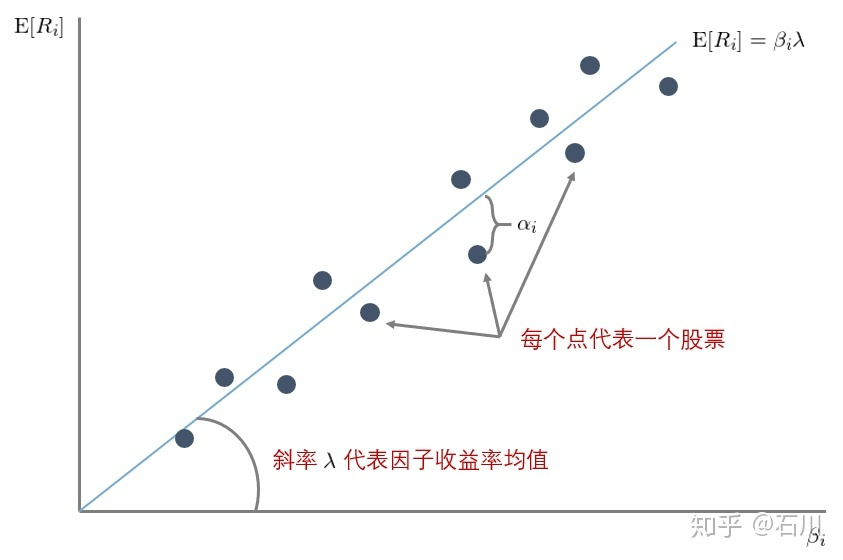
\includegraphics[width=0.6\textwidth]{fig/capm-sml.jpg}
    \caption{CAPM:Security Market Line}
    \label{fig:capm-sml}
\end{figure}

需要注意的是在这里使用$\E[\bm{R_i^e}]$代表资产的预期超额收益率,而非如CAPM中表示的$\E[R_i] - R_f$,这是由于在实证研究中经常使用构建多空对冲投资组合的方法构建因子,因此无需再减去无风险收益率。另外,学界研究的对象始终为资产的预期超额收益,因此有时将“超额”二字省略。

在实证的过程中,等式两侧并不相等,而存在着定价误差$\alpha_i$(Pricing error)。为资产$i$实际预期收益率,与多因子模型隐含的预期收益率之间差值:
\begin{equation*}
    \E[R_i^e] = \alpha_i + \bm{\beta_{i}' \lambda}
\end{equation*}

定价误差有可能由两方面产生:
\begin{itemize}
    \item 模型设定有误:等式右侧遗漏了重要的因子,当被遗漏因子加入后,定价误差消除
    \item 模型设定无误:由于资产收益的实际数据只是总体中的一个样本,那么误差总是存在的。此时需要通过统计的方法检验误差$\alpha_i$是否显著不为零:
    \begin{itemize}
        \item 若$\alpha_i$并非显著不等于于零,那么定价误差的出现只是样本问题
        \item 若$\alpha_i$\textbf{显著不等于零},则说明可以获得模型都无法解释的超额收益,市场对该资产出现错误定价(Mispricing),从而导致了实际预期收益率与多因子模型下的预期收益率出现偏离
    \end{itemize}
\end{itemize}

\subsection*{SML与CML}

如上所述,CAPM描述的是预期收益率与对于市场因子的风险暴露之间的关系,使用证券市场线(Security market line)可表示为:
\begin{figure}[H]
    \centering
    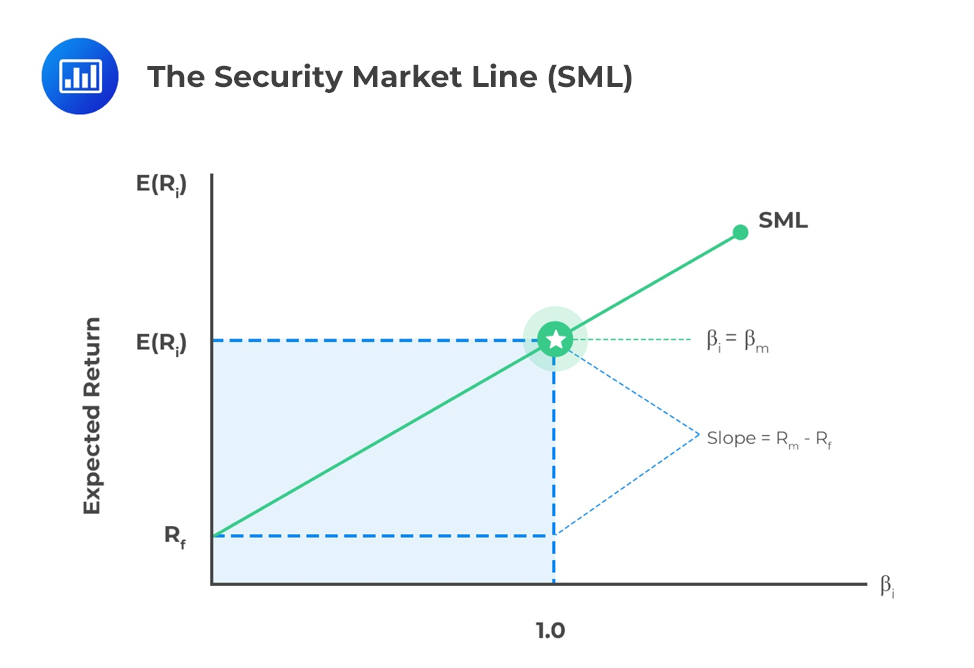
\includegraphics[width=0.8\textwidth]{fig/sml.png}
    \caption{SML}
    \label{fig:sml}
\end{figure}

对于资本市场线(Capital market line,CML)为(Capital allocation line,CAL)的一个特例。在CAL中,该直线由无风险资产($R_f$)与风险资产两种资产组成,而CML中的风险资产为市场组合。那么此时该投资组合的预期收益率为:
\begin{equation*}
    \E(R_P) = w R_f + (1-w) E(R_m)
\end{equation*}

方差有:
\begin{equation*}
    \sigma_P^2 = w^2 \sigma_f^2 + + (1-w)^2 \sigma_m^2 + 2w(1-w) \Cov(R_f,R_m)
\end{equation*}

由于无风险资产风险为零,即$\sigma_f = 0$。并且无风险资产与风险资产的协方差也应为零,即$\Cov(R_f,R_m)$,可以得到:
\begin{equation*}
    \sigma_p = (1-w) \sigma_m
\end{equation*}

将上述$w$关系代入,可得该投资组合预期收益率与标准差的关系:
\begin{align*}
    \E(R_P) &= w R_f + (1-w) E(R_m) \\
    &= \left(1 - \frac{\sigma_p}{\sigma_m} \right) R_f + \E(R_m) \frac{\sigma_p}{\sigma_m} \\
    &= R_f + \frac{\E(R_m) - R_f}{\sigma_m} \sigma_p
\end{align*}

\begin{figure}[H]
    \centering
    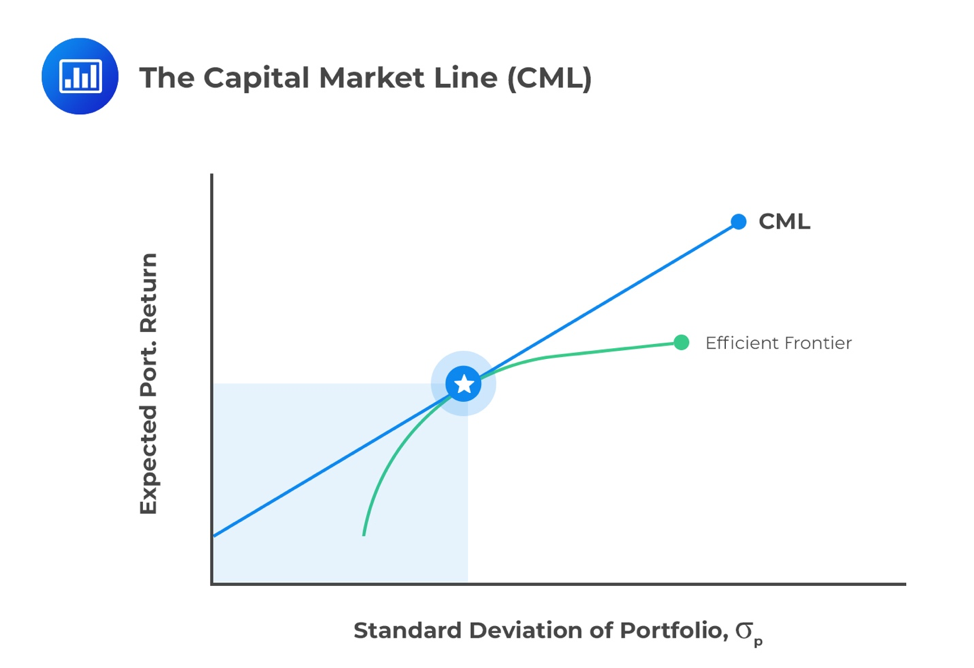
\includegraphics[width=0.8\textwidth]{fig/cml.png}
    \caption{CML}
    \label{fig:cml}
\end{figure}

\subsection{因子、多因子模型与异象}

关于资产$i$预期收益率的多因子关系式,展现了多因子研究中的三个部分:整体$\bm{\beta_{i}' \lambda}$为多因子模型或\uline{定价模型};其中所包含的解释变量即为定价因子(Pricing factors);当对于某个资产$i$,其$\alpha_i$显著不等于零,则这个资产为一个异象(Anomaly),或称之为异象因子(Anomaly factors)。

\begin{equation*}
    \E[R_i^e] = \alpha_i + \bm{\beta_{i}' \lambda}
\end{equation*}

因子描述了众多资产所共同暴露的某种系统性风险,而该因子对应的因子收益率为对该种系统性风险的风险补偿,因子的收益率就是这些资产的共性收益。因此不同的投资组合,归根结底可以归纳为不同因子的组合。由于因子驱动了资产收益率,两者共同运动(Co-movement),因此因子一定与资产收益率的协方差有关。在Fama(1970)中,提出了联合假说(Joint hypothesis)问题,即想要检验市场的有效性就必须先有一个合理的资产定价模型。只有知道了定价模型给出的均衡状态下股票的预期收益率,才有可能检验市场是否有效

因此在多因子模型研究的框架中,面临的的几个主要问题:
\begin{itemize}
    \item 如何选择因子构建多因子模型?
    \item 如何计算资产在因子上的暴露以及因子收益率?
    \item 如何使用统计的方法检验定价误差$\alpha_i$?
\end{itemize}

\subsection{异象}

【待核实】回到定价模型上,如果定价模型无误,且定价误差显著不等于零,那么说明市场存在错误定价,资产为异象。但若定价模型有误,缺少了重要因子,那么即称之为异象因子。

假使我们根据基本面特征或量价指标等特征,挑选出一揽子股票并构建\uline{多空投资组合}。若该投资组合的收益率(方程左侧)无法被多因子模型(方程右侧,如3因子、4因子、5因子模型)解释,则称该特征为一个\textbf{异象}(Anomaly)。即该特征获得了多因子模型无法解释$\alpha$收益率,但从有效市场假说出发,市场中不应该存在很多异象。同时在学界不断的挖掘中,获得了400+个异象,且在样本内都获得了很高的t-statistics,这里可能存在两个原因:
\begin{itemize}
    \item 数据挖掘,大量的异象在样本内被挖掘出,因此Harvey,Liu和Zhu(2016)提出异象收益率的t-statistic至少要超过3.0,而非传统的5\%显著性对应的2.0,才可能真正有效,而非来源于运气
    \item 模型相关,若以$CAPM$为定价模型,那么许多异象都能获得CAPM无法解释的$\alpha$收益率,同时随着定价模型中因子个数的增加,更多的异象变得不再显著,而真正的定价模型是未知的
\end{itemize}

Hou,Xue和Zhang(2017)长达146页对异象的研究中,复现了学术界提出的 447 个异象,涵盖动量(57个)、价值/成长(68个)、投资(38个)、盈利(79个)、无形资产(103个)、以及交易摩擦(102个)六大类。对于这447个异象,在排除了微小市值股票的影响后,其中286个(64\%),在5\%的显著性水平下不再显著(下同)。若按照Harvey,Liu和Zhu(2016)的建议把t-statistic的阈值提升到3.0,其中380个(85\%)异象不再显著。最后,如果使用Hou,Xue和Zhang(2015)提出的4因子模型作为定价模型,那么其中436个(98\%)异象不再显著,仅有 11个异象显著。

对于超额收益,学术界和业界主流的两种解释是错误定价和风险补偿,错误定价意味着投资者可以通过合理的策略获得潜在的超额收益;而风险补偿则意味着投资者获得的收益是以承担额外风险为代价的。

\subsection{因子}

如上所述,不同资产的收益率均可以归结到有限个因子收益率上,不同资产预期收益率的高低由它们对因子的暴露大小决定。因此因子的定义应有:

\begin{quote}
一个因子描述了众多资产共同暴露的某种系统性风险,该风险是资产收益率背后的驱动力;因子收益率正式这种系统性风险的风险溢价或风险补偿,它是这些资产的共性收益。 

\raggedleft{《因子投资》}
\end{quote}

但因子是非常抽象的,如同估值、GDP这些抽象的因子,都可以通过构建\uline{因子模拟投资组合}(Factor mimicking porfolio)的方式,将抽象概念转换为实际载体,从而进行定量研究。构建因子模拟投资组合需要满足两个条件:
\begin{itemize}
    \item 该投资组合在该目标因子上有大于零的暴露、且在其他因子上的暴露为零(纯粹的反应目标因子收益)
    \item 该投资组合的特质性风险(Idiosyncratic risk),即个股收益率在时序上的随机扰动,在所有满足上述条件的投资组合中最小(减少随机扰动带来的误差)
\end{itemize}

第一个条件比较好理解,因为因子模拟投资组合,应该只收到目标因子的驱动,不受其他因子的影响(对于其他因子有因子暴露为零),这才能反应出目标因子的收益。若一个因子投资组合在A与B两个因子上都有较高的暴露,显然难以区分受到什么驱动力的影响。而对于条件二,能构成条件一的投资组合并不唯一,那么由于投资组合是由个股构成,那么应该使得个股的特质性风险最小,即个股在时序上的随机扰动最小,否则将给因子收益率的计算带来较大的误差。

异象有可能能成为优秀的因子,但不是所有异象都是因子。因为作为一个因子(Factor),需要能够解释资产(个股或投资组合)预期收益率截面上的差异,并有增量贡献。具体而言:
\begin{itemize}
    \item 异象从方程的左侧,移动到右侧称为一个因子,称为解释变量,需要考察期是否能解释预期收益率截面上的差异
    \item 由于多个异象之间并不完全独立,需要排除相关性的影响,考察是否有增量贡献
\end{itemize}

许多因子都能解释资产预期收益率截面差异,但显然不能吧所有因子都放进一个多因子模型中。很多因子存在相关性,因此希望因子是相互独立的,每个因子都能对解释资产预期收益率截面差异有显著的增量贡献。如价值因子,也可以采用$E/P$或$B/P$构建High-Minus-Low组合,若同时使用,两者相关性必然很高,因此若使用其一作为价值因子,另一因子对资产预期收益率截面差异的解释能力的增量贡献将变得很低,无法称为因子。另外要考虑简约法则(The Law of Parsimony),每个因子代表的是不同资产所暴露的某种共性风险,那么因子数量一定时有限。学术界主流多因子模型一般包括3~5个因子。目前主流的多因子模型如下:
\begin{itemize}
    \item Fama-French 三因子模型(Fama and French 1993):多因子模型的开山鼻祖,包括MKT、HML以及SMB三因子。其中包含了MKT市场因子,HML价值因子,与SMB规模因子
    \item Carhart 四因子模型(Carhart 1997):在 Fama-French三因子模型上加上了动量MOM因子。
    \item Novy-Marx四因子模型(Novy-Marx 2013):包含MKT,HML,MOM以及PMU四个因子,其中 PMU 所用的财务指标是Gross Profit-to-Asset,代表Profitability维度
    \item Fama-French 五因子模型(Fama and French 2015):Fama和French在其三因子模型的基础上加入了CMA和RMW两个因子,分别代表Investment和Profitability 两个维度。
    \item Hou-Xue-Zhang 四因子模型(Hou, Xue and Zhang 2015):包含MKT,SMB,IVA以及ROE。其中IVA是Total assets的年增长率,代表Investment 维度
    \item Stambaugh-Yuan四因子模型(Stambaugh and Yuan 2016):包含MKT,SMB,MGMT和PERF四个因子。MGMT和PERF分别使用了6个和5个指标,代表Management以及 Performance相关的两个Mispricing因子。虽然该模型只有四个因子,但它用到的基本面和量价指标多达 12 个。
    \item Daniel-Hirshleifer-Sun三因子模型(Daniel, Hirshleifer and Sun 2018):在MKT的基础上,使用PEAD和FIN两个指标作为短期和长期行为因子(Behavioral factors)的代理指标,构建了三因子模型。该模型由于包括了传统的MKT市场因子,又包括行为因子,故称为复合模型。
\end{itemize}

\subsection{因子模型比较}

【待整理】

对于不同多因子模型之间的比较。目前学界主要有三种方法:
\begin{itemize}
    \item GRS tests
    \item Mean-Variance Spanning tests
    \item Bayesian approach
\end{itemize}

GRS tests(Gibbons,Ross和Shanken 1989)检验n个资产在给定因子模型下的定价错误$\alpha$,是否在统计上联合为零(jointly equal to zero)。在比较两个多因子模型时,使用两个模型的因子互为资产和定价模型进行检验。

Mean-Variance Spanning tests考察n个已知资产构建的mean-variance有效前沿能否包含某个新资产(Huberman和Kandel 1987)。在比较两个多因子模型时,使用每个模型的因子构建有效前沿,并逐一检验其能否包含另一个模型中的因子。

在Bayesian approach中,假设比较两个多因子模型$M_1$和$M_2$,数据集使用$D$表示。令 $P(M_1)$和$P(M_2)$为这两个模型的先验概率,且有$P(M_1) + prob(M_2) = 1$(这里假设把多个模型两两比较)。根据贝叶斯定理有:
\begin{equation*}
    P(M_i \given D) = \frac{P(M_i)P(D \given M_i)}{P(M_1)P(D\given M_1) + P(M_2)P(D\given M_2)}
\end{equation*}

其中:
\begin{equation*}
    P(D \given M_i) = \int_{\theta_i} P(\theta_i) P(D \given \theta_i) d\theta_i
\end{equation*}

上式中,$P(\theta_i)$是模型$i$参数的先验分布,$P(D \given \theta_i)$是模型$i$的似然函数。上述贝叶斯方法的核心在于确定$P(\theta_i)$。根据Pastor和Stambaugh(2000)以及Barillas和Shanken(2018)的理论,它和以两个模型中的全部因子作为资产所构成的投资组合的预期最大夏普率的平方与市场夏普率的比值有关。

\subsection{系统性风险}

多因子模型的表达式强调,只有那些影响众多资产收益率共同运动的风险,而非资产的特质性风险(即可以通过分散化规避掉的风险),才是预期收益率的来源。系统性风险(Systematic risk),又称市场风险或不可分散风险,是影响所有资产的、不能通过资产组合而消除的风险。这部分风险是由那些影响整个市场的风险所引起的,无论怎样分散投资,也不可能消除系统性风险。避免集中投资于单一市场可减少系统性风险。单项资产、证券资产组合或不同公司受系统性风险影响不一样,系统性风险的大小通常用beta系数($\beta$系数)来衡量。如上对因子的描述可知,一个因子描述的即为众多资产共同暴露的某种系统性风险,所获得的因子收益率为承受该系统性风险的补偿。

【有疑问】以单因子模型即市场因子为例,有$R_i^e ~ \beta_i MKT$为例,系统性风险是底层的成因,可以有两种理解方式:

似乎并不能在因子模型框架内解释?看秦明的那篇,此时的风险溢酬指$R^e$??

\begin{itemize}
    \item 风险暴露或风险大小$\beta$:对于普通资产,其系统性风险(风险暴露)为正,即$\beta_i = \Cov(R_i,R_M)/\Var(R_M)$为正,即与市场相关性为正,那么暴露的大小决定了最后的超额收益;相反如VIX在美国市场中,与市场相关性为负,那么VIX的系统性风险为负,那么当市场上行时,其收益为负,而当市场下行时,收益为正
    \item 风险溢酬或风险价格$MKT$:【有疑问】系统性风险为正(潜在意思是该资产对系统性风险的暴露为正?),因此有正的风险溢酬;而VIX对于系统性风险的暴露为负,即能降低(对冲)系统性风险,因此负的风险溢酬,或理解为即支付对于市场下行的保费(风险溢酬);作为买方,需要支付更贵的价格(好东西),或获得更低的收益率
    \item 【疑问】意味着正的beta,有正的lambda?负的beta有负的lambda?显然不正确?
    \item 【理解】市场下行风险、市场风险、系统性风险并不等价;系统性风险是最底层,不可知的;市场风险只是系统性风险的一部分,SMB与HML都为对于系统性风险的风险溢酬,市场下行的风险也是系统系风险的一部分?
\end{itemize}

\subsection{股权风险溢价}

股权风险溢价(Equity risk premium)为股票收益与债券收益之差(在CAPM中$R_i-R_f = \beta_i (R_m-R_f)$),大多数时间为正,意味着股票投资比债券投资带来更高的收益,在少数金融危机时可能为负,但投资股票的风险也远大于投资债券。股权溢价之谜(Equity premium puzzle)指在Mebra和Prescott(1985)的研究中,设立模型并最终得到股权溢价的表达式,使用美国实际数据拟合参数,发现需要大的风险厌恶的系数才能拟合实际的数据,而这么大的风险厌恶系数是不合理的。


\subsection{数据处理}

Fama and French (1993)五因子中使用百分比收益,因为设计横截面,投资组合。


\section{随机贴现因子}

\subsection{随机贴现因子与因子模型}

对于资产定价的研究,有两种方式:
\begin{itemize}
    \item 绝对定价(Absolute pricing):试着将资产价格与所暴露的宏观经济风险联系起来,如CCAPM、ICAPM
    \item 相对定价(Relative pricing):利用一系列已知价格的资产给其他资产定价,如期权定价模型或APT
\end{itemize}

而无论采用哪种方式,不同的资产定价模型都可以放入Cochrane(2005)的无套利定价框架之中,资产$i$在$t$时刻的价格$p_{i,t}$应满足如下关系。即在$t+1$时刻,资产处于某种状态$s$,其概率为$\pi_{t+1}(s)$,资产支付的回报和对应的折现因子分别为$\pi_{t+1}(s)$与$m_{t+1}(s)$,此时m为随机贴现因子(Stochastic discount factor,SDF):
\begin{equation*}
    p_{i,t} = \sum_s \pi_{t+1}(s) m_{t+1}(s) x_{t+1}(s)
\end{equation*}

若使用期望表示:
\begin{equation*}
    p_{i,t} = \E_t[m_{t+1}(s) x_{t+1}(s)]
\end{equation*}

或简单写为:
\begin{equation*}
    p = \E[mx]
\end{equation*}

早期的研究重点为研究SDF的性质,以及什么能决定和影响SDF。而如今在的研究,更常见的是通过beta pricing models,即研究资产预期收益率与风险暴露(beta)之间的关系,即熟悉的多因子模型。看似beta pricing models放弃了对SDF的研究,但实际上beta models与SDF是等价的,这种等价性为如今我们能通过多因子模型研究资产定价提供了保证。

根据资产定价理论,随机贴现因子$m$与因子$f$满足关系$m=a+b'f$,将因子$f$通过去均值(demean),使其均值信息保留在$a$中,因此有$m=a+b'(f-\E[f])$。另外,利用$\E[mR^e]=0$,可以将$m$进行缩放,使得$a=1$,得到简化后的关系$m=1+b'(f-\E[f])$。那么此时有如下定理,详见Cochrane(2005)中6.3节:
\begin{thm}
    Given the model:
    \begin{equation}
        m = 1 + [f-\E(f)]'b, \qquad 0=\E(mR^e)
        \tag{6.7}
        \label{cochrane:eq6.7}
    \end{equation}

    one can find $\lambda$ such that
    \begin{equation}
        \E(R^e) \beta' \lambda
        \tag{6.8}
        \label{cochrane:eq6.8}
    \end{equation}

    where $\beta$ are the multiple regression coefficients of excess returns $R^e$ on the factors. Conversely, given $\lambda$ in \ref{cochrane:eq6.8}, we can find b such that \ref{cochrane:eq6.7} holds.
\end{thm}

以上定理说明,当我们吧资产预期超额收益率表示为$\beta$与$\lambda$的乘积(多因子模型)时,SDF可以表示为这些因子的线性组合,此时$\beta$就是资产超额收益$R^e$对于因子f的多元回归系数。

\begin{proof}
    由$m=1+(f-E[f])'b$可知$\E[m]=1$。利用$0=\E[mR^e]$与$\E[m]=1$,以及$\Cov(XY)=E[XY] -\E[X]\E[Y]$可知:
    \begin{align*}
        \Cov(m,R^e) &= \E[mR^e] - \E[m]\E[R^e] \\
        &= 0 - 1 \E[R^e] \\
        &= \E[R^e]
    \end{align*}

    因此$\E[R^e] = -\Cov(m,R^e)$,又由SDF的表达式可知。常数b可以提出,且其他常数不影响协方差可以消去:
    \begin{align*}
        \Cov(m,R^e) &= \Cov(1+(f-\E[f])'b,R^e) \\
        &= \Cov(f'-(\E[f])',R^e)b \\
        &= \Cov(f',R^e)b
    \end{align*}

    因此有:
    \begin{equation*}
        \E[R^e] = -\Cov(f',R^e)b
    \end{equation*}

    利用$\beta' = \Cov(f',R^e)\Var(f)^{-1}$,代入上式:
    \begin{align*}
        \E[R^e] &= -\Cov(f',R^e)\left[ \Var(f)^{-1} \Var(f) \right]b \\
        &= \beta'(-\Var(f)b)
    \end{align*}

    令$\lambda = -\Var(f)b$,则有:
    \begin{equation*}
        \E[R^e] = \beta' \lambda
    \end{equation*}

    这样就从SDF推导得到了多因子模型,而也可以从多因子模型反推出SDF。
\end{proof}

\subsection{随机贴现因子与有效前沿}

有效前沿又称马科维茨的均值-方差前沿(Mean-variance (efficient) frontier),考虑超额收益$R^e$和随机贴现因子$m$,由资产定价理论有$0=\E[mR^e]$:
\begin{align*}
    0 &= \E[mR^e] \\
    &= \E[m]\E[R^e] + \Cov(m,R^e) \\
    &= \E[m]\E[R^e] + \rho(m,R^e)\sigma(m)\sigma(R^e)
\end{align*}

因此有:
\begin{equation*}
    \frac{\E[R^e]}{\sigma(R^e)} = -\frac{\rho(m,R^e)\sigma(m)}{\E[m]}
\end{equation*}

因为相关系数的取值为$0 \leq \rho \leq 1$,因此任意资产的超额收益与SDF应满足如下关系,其被称为Hansen-Jagannathan bound(详见Hansen and Jagannathan(1991)):
\begin{equation*}
    \frac{\abs{\E[R^e]}}{\sigma(R^e)} \leq \frac{\sigma(m)}{\E[m]}
\end{equation*}

若只考虑$\E[R^e]>0$的资产,那么可以得到:
\begin{equation*}
    \frac{\E[R^e]}{\sigma(R^e)} \leq \frac{\sigma(m)}{\E[m]}
\end{equation*}

等式左侧为夏普比率,那么意味着资产的夏普比率有上限。观察上式,当等号成立时,即$\rho(m,R^e)=-1$时,夏普比率最大。此时也意味着该资产在mean-variance frontier之上(由于这些资产夏普比率最大),且这些资产都与SDF完全负相关($\rho=-1$),因此这些资产自身都是完全正相关($\rho=1$)。

\begin{figure}[H]
    \centering
    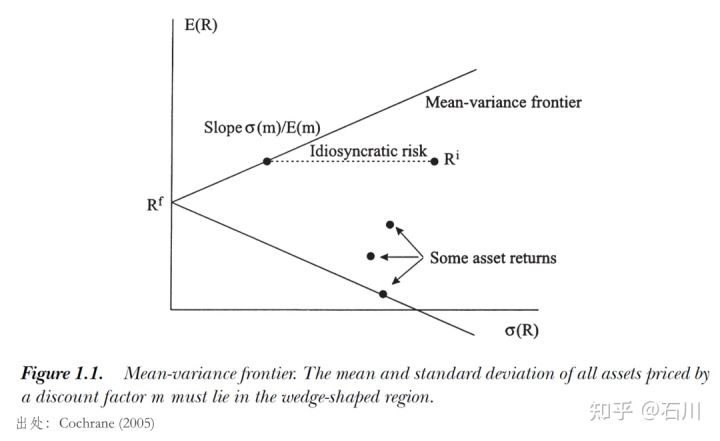
\includegraphics[width=0.8\textwidth]{fig/mean-variance-frontier.jpg}
    \caption{均值方差(有效)前沿}
    \label{fig:mean-variance-frontier}
\end{figure}

那么这种相关性意味着SDF和位于Mean-variance frontier之上的任意资产收益率(记为$R^{mv}$)的等价关系:
\begin{equation*}
    m = a + bR^{mv}
\end{equation*}

在Cochrane(2005)中6.2节中:
\begin{thm}
    There is a discount factor of the form $m = a + bR^{mv}$ if and only if $R^{mv}$ is on the mean-variance frontier, and $R^{mv}$ is not the risk-free rate. (When there is no risk-free rate, if $R^{mv}$ is not the constant-mimicking portfolio return.)
\end{thm}

假设无风险资产存在,则mean-variance frontier是通过$R_f$和tangency portfolio的直线,其之上的任意非无风险资产都可以用来构建SDF,利用SDF和mean-variance frontier的等价关系,可以得到特殊的单因子模型:
\begin{equation*}
    \E[R^e] = \beta \lambda_{R^{mv}}
\end{equation*}

其中$\lambda_{R^{mv}}$为$R^{mv}$的风险溢酬,那么$\beta$为资产超额收益率对均值方差(有效)前沿上资产超额收益的回归系数。同时利用SDF与多因子模型的等价性,以及SDF与均值方差(有效)前沿的等价性,\uline{意味着均值-方差(有效)前沿上资产的收益率嫩能够表示为多因子模型中因子收益率的线性组合。}

\section{投资组合排序法}

\subsection{因子收益率}

如上所述,构建因子模拟投资组合,即获得因子收益率,需要知道所有股票在该因子上的暴露。即因子暴露是,构建因子模拟投资组合,计算因子收益率的前提。而个股在某因子$k$上的暴露为,在控制其他因子之后,该目标因子$k$的收益率与股票超额收益的敏感程度。即需要已知因子收益率才能计算因子暴露。这样就陷入了“先有鸡还是先有蛋”的困境。

而使用排序法(Portfolio sort)可以避免这样的困境,排序法的核心思想在于使用个股在该变量(因子)上的取值大小,来代替个股在该因子上暴露的高低。需要注意其中并没有假设两者之间满足某种特定的数学关系,仅假设变量与因子暴露是相关联的。即假设高BM取值的股票,在围绕BM构建的价值因子上暴露更高,相反,低BM的股票在围绕BM构建的价值因子上的暴露更低。

如公司财务信息如股票估值、市值、盈利等为最主流的一类因子,称为股票风格因子(Style factor),而围绕GDP的这类经济数据构建的因子这称为宏观经济因子。从此可以看出,排序法仅适用于风格因子,因为对于宏观经济因子,很难从股票自身出发,找到与该变量的联系。可以理解为,风格因子对应了个股自身属性,而宏观经济因子为外在环境,很难再个股自身找到对应。因而不适用与排序法。排序法大致可分为如下三个步骤:
\begin{itemize}
    \item 排序:确定股票池,并将其中全部股票在截面上按照排序变量的高低取值进行排序
    \item 分组:按排名高低将全部股票分为N组,做多排名最高的第一组股票,做空排名最低的最后一组股票,从而构建一个多空对冲组合,或称为价差组合(Spread portfolio)。价差组合的收益率即为变量取值最高的$1/N$支股票的收益率,与变量取值最低的$1/N$支股票收益率之差,即围绕该变量构建的\uline{因子收益率}。还需要注意两点,首先,做多组合,与做空组合应该是资金中性的(Dollar neutral),即两个投资组合的金额相同。其次由于多、空组合都包含多支股票,因此需要对个股进行加权,一般有市值加权与等权重两种方法。
    \item 更新:由于个股在因子上的暴露是随着时间变化的,因此需要定期重复进行上述排序、分组两步,完成对因子模拟投资组合的更新,在学术上也称为再平衡(Rebalance),频率一般为每月或每年。计算当前时刻至下一个再平衡时刻的收益率,如此往复,就可以得到因子收益率的时间序列
\end{itemize}

【思考】如上所述,因子收益率是所有股票共性的收益来源,不同股票在在这些因子收益率上的暴露不同,从而造成了截面上的差别。如果只考虑如BM这样的变量,并不能作为所有共性的部分。在Barra中直接作为暴露?需标准化处理

\subsection{检验}

检验因子预期收益率,原假设为因子预期收益率为零,而由定义可知因子的预期收益率应大于零。令$\{\lambda_t\} \; (t=1,2,\dots,T)$代表因子收益率时间序列,因子预期收益率的估计$\hat{\lambda}$以及其标准误分别为:
\begin{gather*}
    \hat{\lambda} = \frac{1}{T}\sum_{t=1}^{T} \lambda_t \\
    s.e.(\hat{\lambda}) = \frac{\sigma(\lambda_t)}{\sqrt{T}}
\end{gather*}

$\{\lambda_t\}$在时序上取平均值,就得到预期因子收益率的估计,这样即可进行t-检验,满足自由度为$T-1$的t分布:
\begin{equation*}
    t\text{-statistic} = \frac{\hat{\lambda}}{s.e.(\hat{\lambda})}
\end{equation*}

\subsection{多重排序法}

上述使用单一变量对股票排序的方法,称之为单变量排序(Univariate sorting)。例如以账面市值比(book-to-market ratio,BM)为例,即为市净率的倒数,学术惯例称其为价值因子而非估值因子。显然BM越高的股票,估值越低,因此价值越高。虽然进行单变量排序,做多BM最高组,做空BM最低组,能极大消除除了BM之外的影响因素。但假如高BM的股票都是大市值、低BM的股票都是小市值,那么就造成了估计误差,使得难以准确估计BM因子。根据上述因子模拟投资组合的所需满足的条件,其应该仅在目标因子上有暴露,在非目标因子上没有暴露。因此为了排除其他因子的干扰,常见的做法时使用多个变量,进行双重排序(Double sorting或Bivariate sorting)或三重排序(Triple sorting),这些方法统称为多重排序法。

根据排序过程中先后或依存的关系,又可分为独立双重排序(Independent double sorting或Unconditional double sorting),或条件双重排序(Dependent double sorting或Conditional double sorting)。例如在Fama and French(1993)中就使用了BM和市值两个指标,进行$2 \times 3$的独立双重排序,其分组方法如下所示:

\begin{table}[H]
\centering
\begin{tabular}{@{}cccc@{}}
\toprule
& \textbf{High(高BM)} & \textbf{Middle(中间组)} & \textbf{Low(低BM)} \\ \midrule
\textbf{Small(小市值)} & S/H & S/M & S/L \\
\textbf{Big(大市值)}   & B/H & B/M & B/L \\ \bottomrule
\end{tabular}
\end{table}

在每一期,都分别独立的将股票划分为$2 \times 3$组,一共得到6个投资组合,常见做法是取这两个变量的各自分位数(Quantile)进行分组。在Fama and French(1993)中,其实用NYSE中位数作为市值分组的依据,而对于BM分组,则采用30\%与70\%的分位数作为依据。每组中的股票收益率按市值加权,得到六个投资组合,并通过如下方法构建规模(市值)和价值(BM)两个因子。与单变量排序相同,在每个变量维度,构建多空组合,即高(收益组合)减低(收益组合)。对于规模因子(SMB)而言,即利用分组,使用小市值组合(Small)减去(Minus)大市值(Big):
\begin{align*}
    SMB &= \frac{1}{3}(S/H + S/M + S/L) - \frac{1}{3}(B/H + B/M + B/L) \\
    &= \frac{1}{3}(S/H-B/H) + \frac{1}{3}(S/M-B/M) + \frac{1}{3}(S/L-B/L)
\end{align*}

而对于估值因子(HML),同样利用分组,使用高BM组合(High)减去(Minus)低BM组合(Low):
\begin{align*}
    HML &=  \frac{1}{2}(S/H + B/H) - \frac{1}{2}(S/L + B/L) \\
    &= \frac{1}{2}(S/H-S/L) + \frac{1}{2}(B/H-B/L)
\end{align*}

如上所述,多重排序法是为了排除非目标因子的干扰。使用双重排序(排序变量$X_1$与$X_2$),学者们也同时考察已有因子的每组内,异象因子是否能解释股票收益率的截面差异。如要检验$X_1$是否能构建异象,还应该考察在$X_2$每组内,根据$X_1$划分的多空组合收益率是否显著。另外独立双重排序可能还存在使得某些组包含股票过少的问题,而使用\uline{条件双重排序}可以解决这个问题。条件双重排序与独立双重排序最大的不同,是按照给定的先后顺序进行排序,如先将$X_1$划分为3组,而后再在$X_1$每组之内,对$X_2$进行划分,最终得到$3\times 2$组,这样保证了每组内有足够的股票。

条件双重排序,核心为考察控制了$X_1$之后,变量$X_2$对股票收益率的影响。此时两个变量的重要性与排序的先后顺序有关,由于第一排序变量仅为控制变量,而第二排序变量与收益率之间的关系更为重要。因此也只需围绕第二排序变量,构建因子模拟投资组合,并计算因子收益率,方法与计算独立双重排序时相同。回到规模和价值的例子中,假设分为$10 \times 10$个投资组合,对于任意一组规模十分组中,在依然进行构建价值多空组合。

\section{多因子模型回归检验}

假设N与K代表资产和因子的个数,对于多因子截面关系式:
\begin{equation*}
    \E[R_{i}^{e}] = \alpha_i + \bm{\beta_{i}' \lambda}
\end{equation*}

在上述截面关系式中,$R_{i}^{e}$为资产i的超额收益率(或直接记作$R_{i}$),$\bm{\beta}_i$为资产i在K个因子上的因子暴露向量,$\bm{\lambda}$为K个因子的收益率向量。\uline{多因子模型研究的核心问题是资产预期收益率在截面之间为什么有差异}。由上式可见,其并不关心时序上的波动,只关心超额收益率的期望$\E[R_{i}^{e}]$与$\bm{\beta}_i$之间截面上的关系(收益与风险)。因子代表了收益率的一种结构(线性关关系),结构一旦确定,资产的收益率就由因子暴露决定,暴露高,收益率就高。

目标是找到一种好的因子结构,使得个股在截面上的预期收益率区分度高,并且使得模型不能解释的定价误差$\alpha_i$尽可能小。若能够在统计上证明所有股票的$\alpha_i$都接近零,这说明这样的因子结构能够较好的解释个股截面预期收益率的差别。因此,多因子模型的回归检验中的重中之重,就是所有$\alpha_i$联合起来是否在统计上足够接近零。

因此,多因子模型的回归检验可以总结为:
\begin{itemize}
    \item 选择因子,并计算每个资产在这些因子上的暴露$\bm{\beta}_i$
    \item 找到个股超额收益率均值$\E[R_{i}]$和因子暴露$\beta_i$在截面上的关系,即进行回归分析
    \item 计算个股的定价误差$\alpha_i$,联合检验这些$\alpha_i$是否在统计上为零
    \item 检验每个因子的预期收益率$\lambda_k$
\end{itemize}

下文所有向量都为列向量,其转置为行向量。
\begin{equation*}
    \underset{\scriptscriptstyle{(N \times 1)}}{\bm{a}}
    = \begin{bmatrix} a_1 \\ a_2 \\ \vdots \\ a_N \end{bmatrix}
    \qquad
    \underset{\scriptscriptstyle{(1 \times N)}}{\bm{a}'}
    = \begin{bmatrix} a_1 & a_2 & \dots a_N \end{bmatrix}
\end{equation*}

\subsection{时序回归}

时间序列回归(Time-series regression)最为简单直接,Black等(1972)最早使用其来检验CAPM。使用因子收益率作为自变量,以资产的超额收益率作为因变量。如上文所述的风格因子,使用排序法构建的因子模拟投资组合,其收益率如经典的HML,SMB等,那么此时可以通过时序回归,来分析个股超额收益率$\E[R_i]$与因子暴露$\beta_i$之间在截面上的关系。由于宏观经济因子难以使用排序法构建因子模拟投资组合并计算其收益率,难以使用时序回归。

对于资产i,进行时间序列回归,即:
\begin{equation*}
    R_{i,t}^{e} = \alpha_i + \bm{\beta}_{i}' \bm{\lambda}_t + \varepsilon_{i,t} \ilsep t=1,2,\dots,T
\end{equation*}

当有N个资产和K个因子时,在$\bm{\lambda}$前加入单列常数1为截距,矩阵形式有:
\begin{equation*}
    \underset{\scriptscriptstyle{(T \times N)}}{\bm{R}}
    = \underset{\scriptscriptstyle{\left(T \times (K+1)\right)}}{\bm{\lambda}}
    \underset{\scriptscriptstyle{\left((K+1) \times N\right)}}{\hat{\bm{\beta}}} 
    + \underset{\scriptscriptstyle{(T \times N)}}{\bm{\epsilon}}
\end{equation*}

其中:
\begin{gather*}
    \bm{R} = \begin{bmatrix} \bm{R}_1 & \dots & \bm{R}_N \\ \end{bmatrix}
    = \begin{bmatrix} R_{1,1} & \dots & R_{1,N} \\ \vdots & \vdots & \ddots \\ R_{T,1} & \dots & R_{T,N} \end{bmatrix} \\
    \bm{\lambda} = \begin{bmatrix} \bm{\lambda}_{1}' \\ \vdots \\ \bm{\lambda}_{T}' \end{bmatrix}
    = \begin{bmatrix} 1 & \lambda_{1,1} & \dots & \lambda_{1,K} \\ \vdots & \vdots & \ddots & \vdots \\ 1 & \lambda_{T,1} & \dots & \lambda_{T,K} \end{bmatrix} 
    \\
    \hat{\bm{\beta}}
    = \begin{bmatrix} \hat{\bm{\beta}}_{0}' \\ \hat{\bm{\beta}}_{1}' \\ \vdots \\ \hat{\bm{\beta}}_{K}' \end{bmatrix}
    = \begin{bmatrix} \hat{\beta}_{0,1} & \dots & \hat{\beta}_{0,N} \\ \hat{\beta}_{1,1} & \dots & \hat{\beta}_{1,N} \\ \vdots & \ddots & \vdots \\ \hat{\beta}_{K,1} & \dots & \hat{\beta}_{K,N} \end{bmatrix}
    \\
    \bm{\epsilon} = \begin{bmatrix}
        \bm{\epsilon}_1 & \dots & \bm{\epsilon}_N \\
    \end{bmatrix}
    = \begin{bmatrix} \epsilon_{1,1} & \dots & \epsilon_{1,N} \\ \vdots & \vdots & \ddots \\ \epsilon_{T,1} & \dots & \epsilon_{T,N} \end{bmatrix}
\end{gather*}

注意在\verb|Python|中,\verb|statsmodel.OLS|对于多因变量回归(Y为多列)一并回归,与对单因变量(Y为单列)逐列回归结果相同。其中$\bm{\beta}_{0}'$为截距,即为$\bm{\alpha}'$,或可以写为:
\begin{gather*}
    \hat{\bm{\beta}}
    = \begin{bmatrix} \bm{\alpha}' \\ \bm{\beta}_{1}' \\ \vdots \\ \bm{\beta}_{K}' \end{bmatrix}
    = \begin{bmatrix} \alpha_{1} & \dots & \alpha_{N} \\ \beta_{1,1} & \dots & \beta_{1,N} \\ \vdots & \ddots & \vdots \\ \beta_{K,1} & \dots & \beta_{K,N} \end{bmatrix}
\end{gather*}

这样就获得了全部资产$i=1,\dots,N$在因子上的暴露向量$\hat{\bm{\beta}}_i$,截距$\hat{\alpha}_i$以及残差$\hat{\bm{\epsilon}}_i$。由于对资产i在时序上进行回归,那么对$R_{t,i}$与$\lambda_t$在时序上取均值,得到$\E_T[R_{t,i}]$和$\E_T[\bm{\lambda_t}]$。因此对于每个资产i,都有如下关系:
\begin{equation*}
    \E_T[R_i] = \alpha_i + \bm{\beta_{i}'} \E_T[\bm{\lambda_t}] \ilsep i=1,2,\dots,N
\end{equation*}

事实上,当自变量为因子收益率时,仅靠对个资产进行时序回归,就可以获得所有资产在截面上的关系。为方便理解,假设单因子情形进行作图,图中红线为$\E_T[R_i] = \beta_i \E_T[\lambda_t]$,那么对于N个资产,每个资产i都对应图上$(\beta_i,\E[R_i])$一点,此时斜率为因子收益率$\hat{\lambda}=\E_T[\lambda_t]$。将当$\beta_i=0$时,即暴露为0,与$\beta_i=1$代入,暴露为1,为因子投资组合。可知该直线过$(0,0)$与$(1,\hat{\lambda})$两点。而时序回归得到的截距$\alpha_i$即为资产i的定价误差,即为此时各个资产到该直线的距离。Black,Jensen和Scholes(1972) 基于如上的论述给出了时序回归法中求解因子预期收益率的简单方法,因子收益率$\bm{\lambda}_t$,在时序上的均值就是因子的预期收益率$\hat{\bm{\lambda}} = \E_T[\bm{\lambda_t}]$。

\begin{figure}[H]
    \centering
    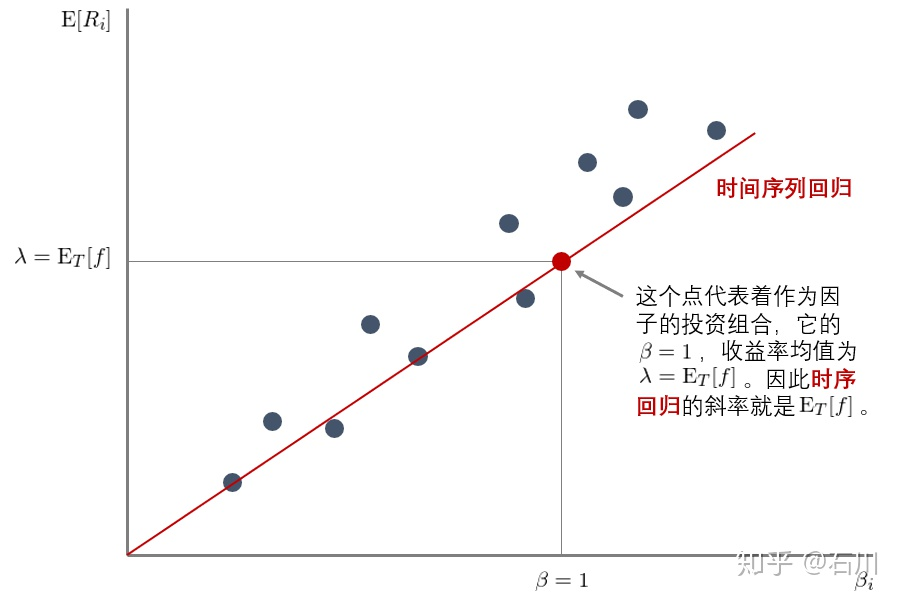
\includegraphics[width=0.8\textwidth]{fig/ts-reg.jpg}
    \caption{时序回归}
    \label{fig:ts-reg}
\end{figure}

这样就通过了时序回归,得到了个股超额收益率与因子暴露在截面上的关系。注意,此时的截面关系并非通过OLS得到,因此直线并不是最小化定价误差$\alpha_i$的平方和为目标求出的。由于是在时序上进行OLS回归,因此其最小化资产i,在时序上的误差$\epsilon_{t,i}$的平方和。

对于检验$\alpha_i$联合起来是否统计上为零,若残差不相关和同方差,标准误可以由OLS标准公式计算。若残差满足独立同分布且为正态分布,可以使用GRS检验,由Gibbons
,Ross和Shanken(1989)提出。而当残差之间存在相关性或者异方差,则需要使用GMM才能得到准确的估计以及标准误,GMM由Lars Peter Hansen于1982年提出。

\subsection{截面回归}

时序回归虽然方便,但仅限于处理股票风格类因子,因子收益率为已知。相比于时序回归,截面回归的优势是,因子的选择范围更广,可以为GDP、CPI、利率等宏观经济指标,可以处理因子收益率时间序列收益率未知的情形。

\subsubsection{方法}

与时序回归相同,第一步仍然需要确定因子暴露$\bm{\beta}$,假设在t时刻,K因子的取值为:
\begin{equation*}
    \bm{F}_t =
    \begin{bmatrix}
        F_{1,K} \\
        F_{2,K} \\
        \vdots \\
        F_{t,K} 
    \end{bmatrix}
\end{equation*}

那么此时,对于资产i,进行时序回归应有:
\begin{equation*}
    R_{i,t} = a_i + \hat{\bm{\beta}}_{i}' \bm{F}_t + \varepsilon_{i,t} \ilsep t=1,2,\dots,T
\end{equation*}

由于此时的解释变量$\bm{F_t}$并非因子收益率,因此截距$a_i$并非定价误差。当有N个资产和K个因子时,在$\bm{\lambda}$前加入单列常数1为截距,矩阵形式有:
\begin{equation*}
    \underset{\scriptscriptstyle{(T \times N)}}{\bm{R}}
    = \underset{\scriptscriptstyle{\left(T \times (K+1)\right)}}{\bm{F}}
    \underset{\scriptscriptstyle{\left((K+1) \times N\right)}}{\hat{\bm{\beta}}} 
    + \underset{\scriptscriptstyle{(T \times N)}}{\bm{\epsilon}}
\end{equation*}

其中:
\begin{gather*}
    \bm{R} = \begin{bmatrix} \bm{R}_1 & \dots & \bm{R}_N \\ \end{bmatrix}
    = \begin{bmatrix} R_{1,1} & \dots & R_{1,N} \\ \vdots & \vdots & \ddots \\ R_{T,1} & \dots & R_{T,N} \end{bmatrix} \\
    \bm{F} = \begin{bmatrix} 1 & \bm{F}_{1}' \\ \vdots & \vdots \\ 1 & \bm{F}_{T}' \end{bmatrix}
    = \begin{bmatrix} 1 & F_{1,1} & \dots & F_{1,K} \\ \vdots & \vdots & \ddots & \vdots \\ 1 & F_{T,1} & \dots & F_{T,K} \end{bmatrix} 
    \\
    \hat{\bm{\beta}}
    = \begin{bmatrix} \hat{\bm{a}}' \\ \hat{\bm{\beta}}_{1}' \\ \vdots \\ \hat{\bm{\beta}}_{K}' \end{bmatrix}
    = \begin{bmatrix} \hat{a}_{1} & \dots & \hat{a}_{N} \\ \hat{\beta}_{1,1} & \dots & \hat{\beta}_{1,N} \\ \vdots & \ddots & \vdots \\ \hat{\beta}_{K,1} & \dots & \hat{\beta}_{K,N} \end{bmatrix}
    \\
    \bm{\epsilon} = \begin{bmatrix}
        \bm{\epsilon}_1 & \dots & \bm{\epsilon}_N \\
    \end{bmatrix}
    = \begin{bmatrix} \epsilon_{1,1} & \dots & \epsilon_{1,N} \\ \vdots & \vdots & \ddots \\ \epsilon_{T,1} & \dots & \epsilon_{T,N} \end{bmatrix}
\end{gather*}

得到了个股因子暴露$\beta$之后,就可以进行第二步截面回归。此时等式左边为$\E_T[R_i]$为整个T其的收益率均值,而右侧为时序回归得到的$\bm{\beta_i}$。对于N个资产,每个资产i都对应点$(\bm{\beta_i},\E[R_i])$。此时对所有资产,进行截面回归:
\begin{equation*}
    \E_T[R_i] = \hat{\bm{\beta}}_{i}' \bm{\lambda} + \alpha_i \ilsep \forall i=1,2,\dots,N
\end{equation*}

矩阵形式应有:
\begin{equation*}
    \underset{\scriptscriptstyle{(N \times 1)}}{\E_T\left[\bm{R}\right]}
    = \underset{\scriptscriptstyle{(N \times K)}}{\hat{\bm{\beta}}'}
    \underset{\scriptscriptstyle{(K \times 1)}}{\bm{\lambda}}
    + \underset{\scriptscriptstyle{(N \times 1)}}{\bm{\alpha}}
\end{equation*}

其中:
\begin{gather*}
    \E_T\left[\bm{R}\right] = \begin{bmatrix} \E_T[R_1] \\ \vdots \\ \E_T[R_N] \end{bmatrix}
    \qquad
    \hat{\bm{\beta}}'
    = \begin{bmatrix} \hat{\bm{\beta}}_{1}' \\ \vdots \\ \hat{\bm{\beta}}_{N}' \end{bmatrix}
    = \begin{bmatrix} \hat{\beta}_{1,1} & \dots & \hat{\beta}_{1,K} \\ \vdots & \ddots & \vdots \\ \hat{\beta}_{N,1} & \dots & \hat{\beta}_{N,K} \end{bmatrix}
    \\
    \bm{\lambda} = \begin{bmatrix} \lambda_{1} \\ \vdots \\ \lambda_{K} \end{bmatrix}
    \qquad
    \bm{\alpha} = \begin{bmatrix} \alpha_1 \\ \dots \\ \alpha_N \end{bmatrix}
\end{gather*}

注意,此时截面回归的残差为定价误差$\alpha_i$,但由于只进行了一次回归,因此只能得到\uline{单组}定价误差$\bm{\alpha}$与\uline{单组}因子预期收益率$\bm{\lambda}$。并且在进行截面回归时没有加入截距项的原因为,多因子模型假设不存在模型设定偏误,资产的预期收益率应仅由因子暴露和因子预期收益率决定。但又如Cochrane(2005)中所指出,也可以考虑包含截距项$\bm{\gamma}_t$的回归模型:
\begin{equation*}
    \E_T[R_{i}] = \bm{\gamma}_i + \hat{\bm{\beta}}_{i}' \bm{\lambda} + \alpha_{i} \ilsep \forall i=1,2,\dots,N
\end{equation*}

\begin{figure}[H]
    \centering
    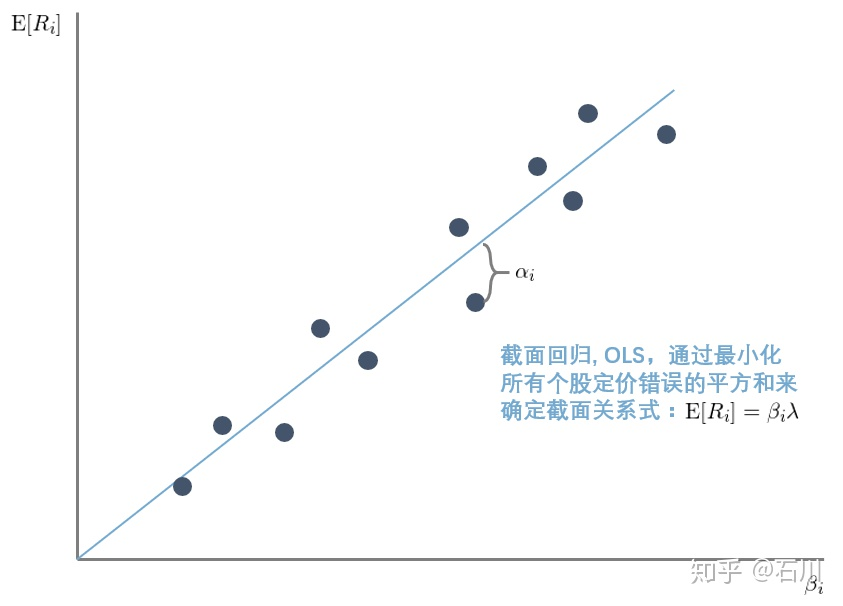
\includegraphics[width=0.8\textwidth]{fig/cs-reg.jpg}
    \caption{传统截面回归}
    \label{fig:cs-reg}
\end{figure}

因此截面回归,也称为两步回归估计(Two-pass regression estimate)。首先,通过时序回归首先得到个股对因子的暴露。其次,对超额收益率取均值,即个股转换为点$(\beta_i,\E[R_i])$,并对N支个股同时进行截面回归,最终得到定价误差与因子收益率,因此截面回归通过最小化所有资产定价误差$\alpha_i$平方和的方式来确定截面关系。

\subsubsection{检验}

对于因子收益率与定价误差,估计量有:
\begin{align*}
    \hat{\bm{\lambda}} &= \left( \hat{\bm{\beta}}' \hat{\bm{\beta}}\right)^{-1} \hat{\bm{\beta}}' \E_T[\bm{R}] \\
    \hat{\bm{\alpha}} &= \E_T[\bm{R}] - \hat{\bm{\beta}} \hat{\bm{\lambda}}
\end{align*}

为了检验每个因子的预期收益率,与联合检验所有资产的定价误差,还需要知道两者的标准误。令$\bm{\epsilon}_t = \begin{bmatrix} \epsilon_{1,t} \\ \vdots \\ \epsilon_{N,t} \end{bmatrix}$为时序回归中的随机扰动,并定义$\bm{\Sigma}_F = \Cov(\bm{F}_t)$与$\bm{\Sigma} = \Cov(\bm{\epsilon}_t)$,利用$\bm{F}_t$与$\bm{\epsilon}_t$之间相互独立,且在各自时序上满足独立同分布,在Cochrane(2005)中给出了$\hat{\bm{\lambda}}$和$\hat{\bm{\alpha}}$的协方差矩阵:
\begin{align*}
    \Cov(\hat{\bm{\lambda}}) &= \frac{1}{T} \left[ \left(\hat{\bm{\beta}}'\hat{\bm{\beta}}\right)^{-1} \hat{\bm{\beta}}' \bm{\Sigma} \hat{\bm{\beta}} \left(\hat{\bm{\beta}}'\hat{\bm{\beta}}\right)^{-1} + \bm{\Sigma}_{F} \right] \\
    \Cov(\hat{\bm{\alpha}}) &= \frac{1}{T} \left[ \bm{I} - \hat{\bm{\beta}} \left(\hat{\bm{\beta}}'\hat{\bm{\beta}}\right)^{-1} \hat{\bm{\beta}}' \right] \bm{\Sigma} \left[ \bm{I} - \hat{\bm{\beta}} \left(\hat{\bm{\beta}}'\hat{\bm{\beta}}\right)^{-1} \hat{\bm{\beta}}' \right]'
\end{align*}

由于真实的$\bm{\Sigma}$与$\bm{\Sigma}_F$未知,采用残差向量$\hat{\bm{\epsilon}}_t = \begin{bmatrix} \hat{\epsilon}_{1,t} \\ \vdots \\ \hat{\epsilon}_{N,t} \end{bmatrix}$代替$\bm{\epsilon}_t$,用样本协方差矩阵$\hat{\bm{\Sigma}}_F$代替$\bm{\Sigma}_F$,将两者的估计值代入上式协方差矩阵中进行计算,就可以计算标准误并进行检验。

由于截面回归的解释变量因子暴露$\hat{\bm{\beta}}_i$并非使用因子收益率回归得到,而是通过时序回归出的估计值,或称为生成的回归变量(Generated regressors),因此在计算标准误时,需要对生成的回归变量造成的误差进行修正。Shanken(1992)给出了修正方法,称为Shanken修正(Shanken correction),即在上述协方差矩阵中加入系数$\left(1 + \bm{\lambda}' \bm{\Sigma}_{F}^{-1} \bm{\lambda} \right)$,则应有:
\begin{align*}
    \Cov(\hat{\bm{\lambda}}) &= \frac{1}{T} \left[ \left(\hat{\bm{\beta}}'\hat{\bm{\beta}}\right)^{-1} \hat{\bm{\beta}}' \bm{\Sigma} \hat{\bm{\beta}} \left(\hat{\bm{\beta}}'\hat{\bm{\beta}}\right)^{-1} \underbrace{\left(1 + \bm{\lambda}' \bm{\Sigma}_{F}^{-1} \bm{\lambda} \right)}_{\scriptscriptstyle{\text{Shanken修正}}} + \bm{\Sigma}_{F} \right] \\
    \Cov(\hat{\bm{\alpha}}) &= \frac{1}{T} \left[ \bm{I} - \hat{\bm{\beta}} \left(\hat{\bm{\beta}}'\hat{\bm{\beta}}\right)^{-1} \hat{\bm{\beta}}' \right] \bm{\Sigma} \left[ \bm{I} - \hat{\bm{\beta}} \left(\hat{\bm{\beta}}'\hat{\bm{\beta}}\right)^{-1} \hat{\bm{\beta}}' \right]' \underbrace{\left(1 + \bm{\lambda}' \bm{\Sigma}_{F}^{-1} \bm{\lambda} \right)}_{\scriptscriptstyle{\text{Shanken修正}}}
\end{align*}

实际计算中使用使用样本$\hat{\bm{\lambda}}$代替$\bm{\lambda}$进行计算。另外除了Shanken修正外,截面OLS回归的另一个问题为,在截面上$\alpha_i$存在相关性,虽然不会影响OLS估计,但将导致使用OLS计算的标准误存在较大误差,低估标准误。因此可以使用广义最小二乘法(Generalized Least Squares,GLS)取代OLS,此时估计量为:
\begin{align*}
    \hat{\bm{\lambda}}_{\text{GLS}} &= \left( \hat{\bm{\beta}}' \bm{\Sigma}^{-1} \hat{\bm{\beta}} \right)^{-1} \hat{\bm{\beta}}' \bm{\Sigma}^{-1} \E_T[\bm{R}] \\
    \hat{\bm{\alpha}}_{\text{GLS}} &= \E_T[\bm{R}] - \hat{\bm{\beta}} \hat{\bm{\lambda}}_{\text{GLS}}
\end{align*}

当使用了GLS并考虑Shanken修正之后,协方差矩阵应有:
\begin{align*}
    \Cov(\hat{\bm{\lambda}}_{\text{GLS}}) &= \frac{1}{T} \left[ \left( \hat{\bm{\beta}}' \bm{\Sigma} \hat{\bm{\beta}} \right)^{-1} \underbrace{\left(1 + \bm{\lambda}_{\text{GLS}}' \bm{\Sigma}_{F}^{-1} \bm{\lambda}_{\text{GLS}} \right)}_{\scriptscriptstyle{\text{Shanken修正}}} + \bm{\Sigma}_{F} \right] \\
    \Cov(\hat{\bm{\alpha}}_{\text{GLS}}) &= \frac{1}{T} \left( \bm{\Sigma} - \hat{\bm{\beta}} \left(\hat{\bm{\beta}}' \bm{\Sigma}^{-1} \hat{\bm{\beta}}\right)^{-1} \hat{\bm{\beta}}' \right) \underbrace{\left(1 + \bm{\lambda}_{\text{GLS}}' \bm{\Sigma}_{F}^{-1} \bm{\lambda}_{\text{GLS}} \right)}_{\scriptscriptstyle{\text{Shanken修正}}}
\end{align*}

那么可以同时使用OLS或GLS检验全部N个定价误差$\alpha_i$是否联合为零,构建如下自由度为$N-K$的$\chi^2$统计检验量:
\begin{align*}
    \text{OLS} \;:\;& \hat{\bm{\alpha}}' \Cov(\hat{\bm{\alpha}})^{-1} \hat{\bm{\alpha}} \sim \chi^2_{N-K} \\
    \text{GLS} \;:\;& \hat{\bm{\alpha}}_{\text{GLS}}' \Cov(\hat{\bm{\alpha}}_{\text{GLS}})^{-1} \hat{\bm{\alpha}}_{\text{GLS}} \sim \chi^2_{N-K}
\end{align*}

检验因子预期收益率$\lambda$,只需要从$\Cov(\hat{\bm{\lambda}})$或$\Cov(\hat{\bm{\lambda}}_\text{GLS})$协方差矩阵中取出对角线元素开放即可,即为K个因子的标准误。对于每个因子k,利用其预期收益率$\hat{\lambda}_k$与其标准误,即可计算出相应的自由度为$T-1$的t-统计量,进行检验。

\subsection{时序回归 vs 截面回归}

对于时序回归而言,通过对因子收益率在时序取均值$\bm{\lambda} = \E_T[\bm{\lambda}_t]$,来得到隐含的截面关系。因此$\E[R_i] = \bm{\beta}_{i}' \bm{\lambda}$必然过原点$(0,0)$,以及因子收益率的投资组合$(1,\bm{\lambda})$($\bm{\beta_i}=1$)。而在截面回归中,因子暴露已经通过时序回归确定,而在第二次进行截面回归时,充分使用了个股数据。若使用OLS进行截面回归,以最小化个股定价误差$\alpha_i$的平方和为目标。因子收益率通过回归得到,与时序中直接通过计算均值的方式不同,更加合理。

\begin{figure}[H]
    \centering
    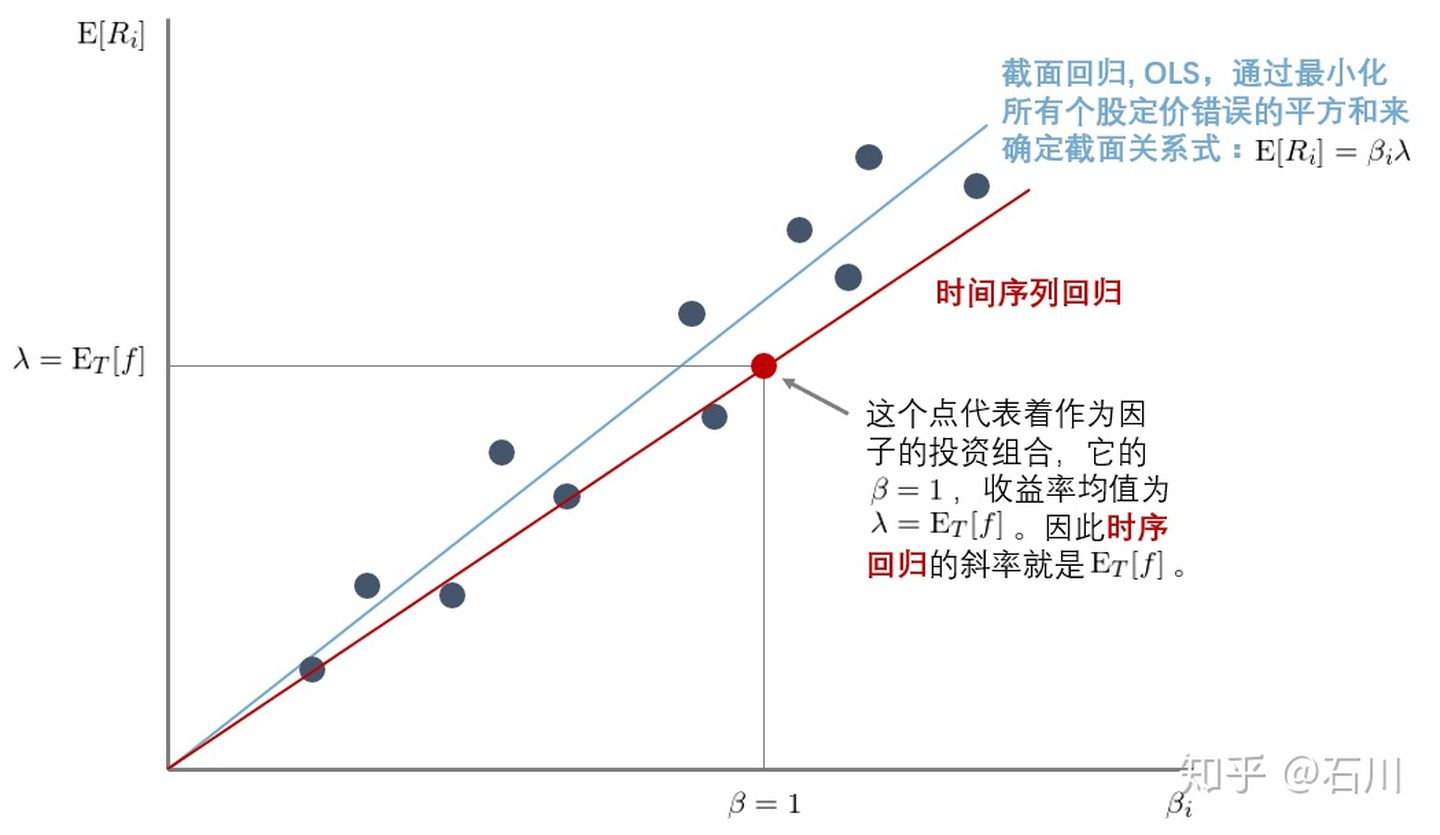
\includegraphics[width=0.8\textwidth]{fig/ts-vs-cs.jpg}
    \caption{时序回归与截面回归}
    \label{fig:ts-vs-cs}
\end{figure}

\subsection{Fama-MacBeth回归}

\subsubsection{方法}

在Fama和MacBeth(1973)中,提出了Fama-MacBeth截面回归,目的是为了检验 CAPM。Fama-MacBeth截面回归也分为两步,因此称为两步回归,但与传统截面回归有所不同。首先,与传统截面回归相同,也需要先进行时序回归,得到资产i超额收益率$R_i$在因子上的暴露$\bm{\beta}_i$。在第一步中,又可分为因子暴露$\bm{\beta}_i$不变与$\bm{\beta}_i$时变两种情形。对于因子暴露不变的情形,对$t=1,\dots,T$整体时序样本,只进行一次时序回归,得到一个不随时间改变的因子暴露。

在Fama和MacBeth(1973)中,采用滚动窗口的方法估计$\bm{\beta_i}$,因此对于不同的t,$\bm{\beta_i}$随时间改变。
\begin{equation*}
    \bm{R}_{i,t} = \bm{a}_i + \bm{\beta_{i} \bm{F}_t + \bm{\varepsilon}_{i,t}} \ilsep \forall t=1,2,\dots,T
\end{equation*}

其次,在传统截面回归中,如上节所述,第二步只进行一次截面回归。即对资产i的超额收益率$\bm{R}_i = \begin{bmatrix} R_{1,i} \\ \vdots \\ R_{T,i} \end{bmatrix}$在时序上取均值得到$\E_T[\bm{R}_i]$,与该资产i的因子暴露$\bm{\beta}_i$进行回归,只进行了\uline{1次回归}:
\begin{equation*}
    \E_T[\bm{R}_i] = \bm{\beta_{i}' \lambda_i} + \bm{\alpha}_i \ilsep \forall i=1,2,\dots,N
\end{equation*}

而在Fama-MacBeth截面回归中,第二步并不对$R_{i,t}$在时序上取均值,需要对在$t=1,\dots,T$期上各进行一次截面回归,一共进行\uline{T次回归},得到T组因子收益率$\bm{\lambda}_t$与T组定价误差$\bm{\alpha}_t$:
\begin{equation*}
    \bm{R}_{i,t} = \bm{\beta}_{i}' \bm{\lambda}_{i,t} + \bm{\alpha}_{i,t} \ilsep \forall i=1,2,\dots,N
\end{equation*}

因子暴露$\hat{\bm{\beta}}$由上一步得到(可为不变或时变)为估计值,以不变为例,对于第t期而言,写为矩阵形式为:
\begin{equation*}
    \underset{\scriptscriptstyle{(N \times 1)}}{\bm{R}_t} = \underset{\scriptscriptstyle{(N \times K)}}{\hat{\bm{\beta}}'} \underset{\scriptscriptstyle{(K \times 1)}}{\bm{\lambda}_t} + \underset{\scriptscriptstyle{(N \times 1)}}{\bm{\alpha}_t}
\end{equation*}

其中:
\begin{gather*}
    \bm{R}_t = \begin{bmatrix}R_{1,t} \\ \vdots \\ R_{N,t}\end{bmatrix}
    \qquad 
    \hat{\bm{\beta}}' = 
    \begin{bmatrix} \hat{\bm{\beta}}_{1}' \\ \vdots \\ \hat{\bm{\beta}}_{N}' \end{bmatrix} =
    \begin{bmatrix} \hat{\beta}_{1,1} & \dots & \hat{\beta}_{1,K} \\ \vdots & \ddots & \vdots \\ \hat{\beta}_{N,1} & \dots & \hat{\beta}_{N,K} \end{bmatrix}
    \\
    \bm{\lambda}_t = \begin{bmatrix}\lambda_{1,t} \\ \vdots \\ \lambda_{K,t} \end{bmatrix}
    \qquad
    \bm{\alpha}_t = \begin{bmatrix}\alpha_{1,t} \\ \vdots \\ \alpha_{N,t} \end{bmatrix}
\end{gather*}

进行T次回归后,可以得到K个因子随时间变化的因子收益率$\bm{\lambda}$,与N个资产随时间变化的定价误差$\bm{\alpha}$:
\begin{gather*}
    \underset{\scriptscriptstyle{K \times T}}{\bm{\lambda}}
    = \begin{bmatrix} \bm{\lambda}_{1}' \\ \vdots \\ \bm{\lambda}_{K}' \end{bmatrix}
    = \begin{bmatrix} \lambda_{1,1} & \dots & \lambda_{1,T} \\ \vdots & \ddots & \vdots \\ \lambda_{K,1} & \dots & \lambda_{K,T} \end{bmatrix}
    \qquad
    \underset{\scriptscriptstyle{N \times T}}{\bm{\alpha}}
    = \begin{bmatrix} \bm{\alpha}_{1}' \\ \vdots \\ \bm{\alpha}_{N}' \end{bmatrix}
    = \begin{bmatrix} \alpha_{1,1} & \dots & \alpha_{1,T} \\ \vdots & \ddots & \vdots \\ \alpha_{N,1} & \dots & \alpha_{N,T} \end{bmatrix}
\end{gather*}

注意,如上所述,若使用滚动方法,即$\bm{\beta}$时变。在实际回归过程中,采用Lead-lag回归的方法,即对于$t$期,使用截止$t-1$期的一段给定窗口的历史数据进行第一步的时序回归,得到估计$\hat{\bm{\beta}}_{i,t-1}$。并且使用其作为第二步$t$期截面回归的解释变量,得到因子收益率:
\begin{equation*}
    R_{i,t} = \hat{\bm{\beta}}_{i,t-1} \bm{\lambda}_t + \alpha_{i,t} \ilsep \forall i=1,2,\dots,N
\end{equation*}

或如Cochrane(2005)中,在截面回归中加入截距项$\gamma_t$:
\begin{equation*}
    R_{i,t}^{e} = \gamma_t + \hat{\bm{\beta}}_{i,t-1} \bm{\lambda}_t + \alpha_{i,t} \ilsep \forall i=1,2,\dots,N
\end{equation*}

Fama-MacBeth截面回归和传统截面回归的相同点和区别是:
\begin{itemize}
    \item FM截面回归与传统截面回归,第一步都需先进行时序回归,以确定个股的因子暴露$\bm{\beta_i}$
    \item 在第二步中,传统截面回归将$R_{i,t}$或$\underset{\scriptscriptstyle{(N \times T)}}{\bm{R}}$在时序上取均值得到$\E_T[R_i]$或$\underset{\scriptscriptstyle{(N \times 1)}}{\E_T\left[\bm{R}\right]}$,再进行1次截面回归,得到整体样本K个因子的因子收益率$\underset{\scriptscriptstyle{(K \times 1)}}{\bm{\lambda}}$与N个资产的定价误差$\underset{\scriptscriptstyle(N \times 1)}{\bm{\alpha}}$
    \item 在第二步中,FM截面回归,在各个不同的t时刻,使用$R_{i,t}$与$\bm{\beta_{i}}$进行回归,得到K个因子时变的因子收益率$\underset{\scriptscriptstyle{(K \times T)}}{\bm{\lambda}}$与N个资产时变的定价误差$\underset{\scriptscriptstyle(N \times T)}{\bm{\alpha}}$。再将回归结果在时序上取均值得到因子收益率$\underset{\scriptscriptstyle{(K \times 1)}}{\hat{\bm{\lambda}}} = \E_T[\bm{\lambda}]$与定价误差$\underset{\scriptscriptstyle{(N \times 1)}}{\hat{\bm{\alpha}}} = \E_T[\bm{\alpha}]$
    \item 即传统回归为先取均值,后回归。而FM回归为先回归,后取均值。因此对于不变的$\beta$值,对于线性模型而言两者的结果相同。
\end{itemize}

\begin{note}
    FM回归注意事项:
    \begin{itemize}
        \item 在计算$\beta$时,一般为同期关系,即同期收益率,与同期的因子收益率进行回归,得到同期的因子暴露
        \item 而在第二步回归中,为领先-滞后关系,即下一期收益率与当期的beta回归,得到下一期的因子溢价的估计
        \item 对于两步回归的截距选择,两步回归中都应考虑截距,第一步若无截距项,即假设没有模型设定问题,这肯定是不现实的,因此应该会提高因子暴露,使得第二步回归后的因子溢价变为显著
        \item 若第二步不考虑截距,即不存在遗漏变量(不现实),在Barra中如CNE6,截距代表的就是A股市场因子
    \end{itemize}
\end{note}

\subsubsection{检验}

对于T期回归之后构成的因子收益率与定价误差的时间序列,在时序上取均值,即可以以此估计定价误差以及因子收益率:
\begin{equation*}
    \hat{\lambda}_k = \frac{1}{T} \sum_{t=1}^{T} \lambda_{k,t}
    \qquad
    \hat{\alpha}_i = \frac{1}{T} \sum_{t=1}^{T} \alpha_{i,t}
\end{equation*}

写为矩阵形式有:
\begin{equation*}
    \hat{\bm{\lambda}} 
    = \begin{bmatrix} \hat{\lambda}_1 \\ \vdots \\ \hat{\lambda}_K \\ \end{bmatrix}
    = \begin{bmatrix} \frac{1}{T} \sum_{t=1}^{T} \lambda_{1,t} \\ \frac{1}{T} \sum_{t=1}^{T} \lambda_{2,t} \\ \vdots \\ \frac{1}{T} \sum_{t=1}^{T} \lambda_{K,t} \\ \end{bmatrix} 
    \qquad
    \hat{\bm{\alpha}} 
    = \begin{bmatrix} \hat{\alpha}_1 \\ \vdots \\ \hat{\alpha}_N \\ \end{bmatrix}
    = \begin{bmatrix} \frac{1}{T} \sum_{t=1}^{T} \alpha_{1,t} \\ \frac{1}{T} \sum_{t=1}^{T} \alpha_{2,t} \\ \vdots \\ \frac{1}{T} \sum_{t=1}^{T} \alpha_{N,t} \\ \end{bmatrix}
\end{equation*}

不同于传统截面回归,只得到$\lambda$和$\alpha$的一个全样本估计,在FM截面回归中得到T个$\lambda$和$\alpha$的样本估计,这样就可以求出两者标准误为:
\begin{align*}
    s.e.(\hat{\lambda}_k) &= \left[ \frac{1}{T^2} \sum_{t=1}^{T} (\hat{\lambda}_{k,t} - \hat{\lambda}_k)^2 \right]^{\frac{1}{2}} \\
    s.e.(\hat{\alpha}_i) &= \left[ \frac{1}{T^2} \sum_{t=1}^{T} (\hat{\alpha}_{i,t} - \hat{\alpha}_i)^2 \right]^{\frac{1}{2}}
\end{align*}

对于$\hat{\bm{\alpha}} = \frac{1}{T} \sum_{t=1}^{T} \hat{\bm{\alpha}}_{t}$与其协方差矩阵有:
\begin{equation*}
    \Cov(\hat{\bm{\alpha}})
    = \frac{1}{T^2} \sum_{t=1}^{T} \left(\hat{\bm{\alpha}}_t - \hat{\bm{\alpha}}\right) \left(\hat{\bm{\alpha}}_t - \hat{\bm{\alpha}}\right)'
\end{equation*}

在有了$\Cov(\hat{\bm{\alpha}})$矩阵之后,便可以使用$\chi^2-$统计量检验全部N个定价误差是否联合为零:
\begin{equation*}
    \hat{\bm{\alpha}}' \Cov(\hat{\bm{\alpha}})^{-1} \hat{\bm{\alpha}} \sim \chi_{N-K}^{2}
\end{equation*}

若在第一步时序回归中$\bm{\beta_i}$不变,那么对于传统截面回归的先均值再回归,与FM截面回归的先回归再均值,两种方式在所有T期上得到的估计是相同的(但FM截面回归在检验上一定的优势)。

【待整理】

一步在时序上进行回归得到,相同的结果?

由于截面上收益率的(上市公司收益,乃至基金收益)相关性显然不会为零,正的截面相关性使得standard error被低估,因此计算t值的时候被高估。FM方法先在每个时间点t,进行截面回归,而后在时序上取对估计值去平均(假设在时序上不相关?)。

Fama-MacBeth回归的最大优点是把T期的回归结果作为T个独立的样本,排除了残差截面相关性对标准误的影响。股票的残差收益率在截面上具有很高的相关性,因此该修正对于准确计算标准误至关重要。

下面来说说它的不足。首先,Fama-MacBeth回归对于残差在时序上的相关性无能为力。如果残差在时序上存在相关性,则需要对Fama-MacBeth回归得到的标准误进一步修正。Petersen(2009)分析了不同的回归技术在分析面板数据(panel data)时由于忽略残差的时序或截面相关性而导致不准确的标准误(低估了其真实值)。这篇文章非常值得一读。其次,上文提到,在截面回归中用到的$\bm{\beta}_i$并不是已知的,而是通过时间序列得到的估计值(generated regressors),因此存在误差。Fama-MacBeth 回归对此也无能为力,需要Shanken correction。

\subsection{Barra多因子模型}

Barra多因子模型也是截面回归模型,其考虑了行业因子和来自基本面和技术面的风格因子。但与传统的截面回归模型不同的是在Barra模型中,因子暴露并非来自时间序列回归,而是直接来自基本面或者技术面数据本身。

例如Book-to-Market ratio,在Fama-French三因子模型中,其被用来构建HML(High-Minus-Low)投资组合,投资组合的收益率作为因子。由时序回归决定个股在这个因子上的暴露,与个股实际的BM无关。但在Barra模型中,BM直接用于确定因子暴露,但需要进行标准化。有了因子暴露,Barra截面模型与传统截面模型相同,都是通过截面回归确定因子收益率。因此,Barra 模型(业界代表)和学术界流行的因子模型最大的不同就是因子暴露$\bm{\beta_i}$的确定。

对于两种确定因子暴露的方法,通过时间序列得到的$\bm{\beta}$,经过平滑,变化更加缓慢。而直接使用基本面数据获得$\bm{\beta}$,可以更快的捕捉公司的变化。需要注意的是,这些因子都需要进行标准化,不能直接使用原始数据。例如,公司市值不经过标准化而作为因子暴露,公司市值差异巨大。假设A公司市值为B公司的100倍,此时显然不能说A公司的超额收益率对于市值因子的暴露为B公司的100倍。所以对于市值因子或其他\uline{风格因子},常见的是首先取对数,然后再进行标准化。对于其他的风格因子,也需要采用相应的标准化处理。在Barra的文档中对如何标准化因子暴露有详细的说明。对于行业因子,Barra将因子暴露处理为Binary变量或虚拟变量,例如工商银行在银行业的暴露为1,而在其他行业的暴露为0。

\subsection{GRS}

\subsection{GMM}

GMM,它可以轻松的求出我们需要的各种量(Hansen 功不可没啊)。另外值得一提的是,在截面回归时用到的$\beta_i$并不是已知、真实的,而是从时间序列回归得出的估计值,它们称为 generated regressors,存在误差。Shanken (1992) 给出了解决该问题的修正方法,称为 Shanken correction。利用 Shanken correction 和 GMM,就可以检验$\alpha$是否为零了。

如今我们有了 GMM 这样的大杀器,能够方便的处理残差的各种相关性。

\subsection{Mean-variance spanning}


\appendix

\begin{appendices}

\section{夏普比率}

在1994年,作者重新定义事前(ex-ante)夏普比率为:
\begin{equation*}
    S_a = \frac{\E[R_a-R_b]}{\sigma_a} = \frac{\E[R_a-R_b]}{\sqrt(\Var (R_a - R_b))}
\end{equation*}

其中$R_a$为资产收益,$R_b$为无风险资产收益,那么此时分子为超额收益的期望,分母则为超额收益标准差,事后(ex-post)夏普比率则使用已实现收益进行计算。根据方差的性质,若在样本期间内认为无风险收益$R_f$为常数,那么此时$\sqrt{\Var[R-R_f]} = \sqrt{\Var[R]}$。

由于收益数据一般为日频或月频的,而最终需要将夏普比率进行年化。因此需要进行一系列的调整。首先,无风险利率一般都是年化以后的,因此在计算超额收益率时,需要将其调整为月频或日频的。

对于无风险利率的使用,中央财经大学资产定价中心使用一年存款利率,日频数据则除以365。石川BetaPlus小组,使用3个月Shibor,日频数据同样除以365。相关利率历史数据可以在万得终端、债券数据库、债券走势分析、货币市场中得到。

【存疑】如面对月频收益率,对应月频无风险利率应为$(1 + r_{monthly}^f)^{12} = 1 + r_{annual}^f$。而对应日频应为$(1 + r_{daily}^f)^{252} = 1 + r_{annual}^f$(虽然债券应为365日计息,但实际如股票等资产交易日只有252),或直接除以天数计算。(对于利率对应天数的选择,应对应具体情况,如果插值就应该对应日历日。若对于无风险利率的计算,相当于吧一年的无风险利率平摊到每个交易日,因此从经济含义上而言不应该使用日历日,而应该使用交易日。)

其次,当计算完日频或月频的夏普比率后,需要将其转化为年化的夏普比率。当收益率为日频,其均值乘以252交易日(或对于中国市场240交易日)进行年化,而对于月频收益率则乘以12,此时实际假定了\uline{年收益为日收益或月收益之和}。当假设日收益或月收益之间相互独立时(协方差为零),方差可加。此时波动率却不随时间线性变化,而是随着时间的平方根变化($\sqrt{t}$)。因此对于日频的夏普比率,应乘以$\frac{252}{\sqrt{252}} = \sqrt{252}$进行转换,而对于月频则同理应乘以$\sqrt{12}$进行转换。还需要注意的是偏度和峰度不随着放大缩小改变,即不受年化的影响。注意:日频或月频的夏普比率转换为年频,与实际年频计算存在一定差距。并且当收益率之间的关系为叠乘关系时,对于$n$期收益率的波动率进行年化,正确的计算波动率的方式为(见波动率章节):
\begin{equation*}
    \sigma_a = \sqrt{ \left[\sigma_n^2 + (1+\mu_n)^2\right]^{n} - (1+\mu_n)^{2n} }
\end{equation*}

\section{APT推导}

第一步,假设资产的收益率,在单因子情形下,满足如下线性模型:
\begin{equation*}
    R_i = \mu_i + \beta_i f + \varepsilon_i \ilsep i =1,\dots,n
\end{equation*}

此时$R_i$为资产收益率,$\mu_i$资产$i$的预期收益率,$\beta_i$是资产在因子上的暴露,而$f$是因子取值,而非因子风险溢酬,$\varepsilon_i$为资产$i$收益率的随机扰动或特质性收益率,并满足$\E[f]=\E[\varepsilon_i]=0$,若改写为向量形式,为Ross在APT中使用的收益率模型,有:
\begin{equation*}
    \bm{R} = \bm{\mu + f\beta + \varepsilon}
\end{equation*}

第二步,构建一个arbitrage portfolio,这个投资组合中资产的权重$\omega$满足如下两点特性。首先,该投资组合是零额投资的,即:
\begin{equation*}
    \bm{w' 1 = 0}
\end{equation*}

其中有$\bm{1}$为全为1的向量。其次,并且$\bm{w'\beta}=0$,即该投资组合在该因子上的暴露为零。此时这个投资组合的收益率应为:
\begin{equation*}
    R_p = \bm{w'R = w'\mu + w'\beta f + w'\varepsilon}
\end{equation*}

由上可知,这个投资组合的收益率可化简为:
\begin{equation*}
    R_p = \bm{w'R = w'\mu} 
\end{equation*}

第三步,运用无套利约束,可知根据$\bm{w}$构建的投资组合有如下性质:零额投资;对因子的暴露为零(因此该组合没有系统性风险);没有特质性风险暴露(因为组合中特质性收益率为零)。换言之,这样一个投资组合,既没有资金投入又没有风险暴露,因此根据无套利约束条件,它的收益率必须为零,即:
\begin{equation*}
    R_p = \bm{w'\mu} = 0
\end{equation*}

根据几何可知,$w' 1 = w' \beta = w'\mu = 0$,说明$\bm{w'}$与$\bm{1}$,$\bm{\beta}$和$\bm{\mu}$,都相互垂直。因此$\bm{\mu}$必然在$\bm{1}$和$\bm{\beta}$构成的平面内。

\begin{figure}[H]
    \centering
    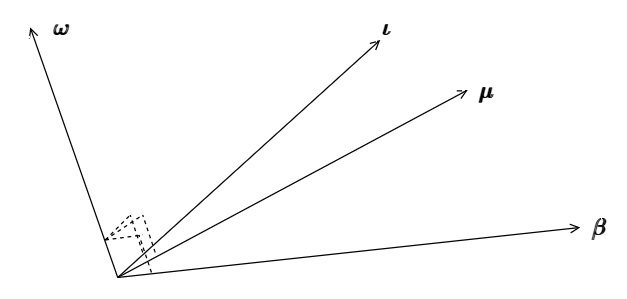
\includegraphics[width=0.6\textwidth]{fig/apt.jpg}
    \caption{APT}
    \label{fig:apt}
\end{figure}

因此在数学上,资产预期收益率$\bm{\mu}$可以写成$\bm{1}$与$\bm{\beta}$的线性组合,即:
\begin{equation*}
    \bm{\mu} = \gamma_1 \bm{1} + \gamma_2 \bm{\beta}
\end{equation*}

那么此时上式应对任何资产都成立,为了求解$\gamma_1$与$\gamma_2$可代入特殊资产,无风险资产($R_f$),与市场组合($R_M$)。由于无风险资产的因子暴露为零,代入上式可得:
\begin{equation*}
    R_f = \gamma_1
\end{equation*}

对于市场组合,其$beta=1$,并将$\gamma_1 = R_f$代入,可得:
\begin{equation*}
    R_M = R_f + \gamma_2 \times \bm{1}
\end{equation*}

因此有:
\begin{equation*}
    \gamma = R_M - R_f
\end{equation*}

代入原式,最终可得到CAPM的表达式:
\begin{equation*}
    \mu_i = R_f + \beta_i(R_M - R_f)
\end{equation*}

在此基础上,扩展至多因子,即得到APT模型:
\begin{equation*}
    \E[R_{i}^{e}] = \mu_i - R_f = \beta_{i,1} \lambda_1 + \beta_{i,2} \lambda_2 + \dots + \beta_{i,K} \lambda_K
\end{equation*}

\section{Campbell-Shiller分解}

Campbell-Shiller分解又称为Campbell-Shiller return identity或Campbell-Shiller log linear relation,对于对数收益($r_{t+1}$)有如下近似关系(忽略常数,$\rho$为常数):
\begin{equation*}
    r_{t+1} \approx \rho(p_{t+1} - d_{t+1}) + \Delta d_{t+1} - (p_t - d_t)
\end{equation*}

因此可以看到未来收益的来源可以分为三个部分:
\begin{itemize}
    \item 未来高的price-dividend ratio,或未来高股价
    \item 股息的增长
    \item 当前低的price-dividend ratio,或现在低股价
\end{itemize}

\begin{proof}
    对于百分比收益率$R_{t+1}$有如下关系,提取$D_{t+1}$并同除$D_{t}$:
    \begin{equation*}
        R_{t+1} = \frac{P_{t+1} + D_{t+1}}{P_t} = \frac{\left( \frac{P_{t+1}}{D_{t+1}} + 1\right) \frac{D_{t+1}}{D_t}}{\frac{P_t}{D_t}}
    \end{equation*}

    对等式两边取对数,令$r_t = \ln(R_t)$,$p_t = \ln(P_t)$与$d_t = \ln(D_t)$,并且令$\delta_t = \ln(\frac{P_t}{D_t})$,则有:
    \begin{align*}
        r_{t+1} &= \ln\left( 1 + \frac{P_{t+1}}{D_{t+1}} \right) + \ln\left( \frac{D_{t+1}}{D_t} \right) - \ln\left( \frac{P_t}{D_t} \right)  \\
        &= \log \left( 1 + e^{\delta_{t+1}} \right) + \Delta d_{t+1} - \delta_t
    \end{align*}

    使用泰勒级数在$x_0$展开$\ln(1+e^x)$,并只保留一次项:
    \begin{equation*}
        \ln(1+e^x) \approx \ln (1+e^{x_0}) + \frac{e^{x_0}}{1+e^{x_0}}(x-x_0)
    \end{equation*}

    若使用长期均值$\delta$作为$x_0$:
    \begin{equation*}
        r_{t+1} \approx \ln(1+e^{\delta}) + \frac{e^{\delta}}{1+ e^{\delta}} (\delta_{t+1} - \delta) + \Delta d_{t+1} - \delta_t
    \end{equation*}
        
    令$\rho = \frac{e^\delta}{1+e^\delta} = \frac{1}{1+D/P}$,则$\kappa = \ln (1+e^\delta) - \rho \delta$两者均为常数:
    \begin{equation*}
        r_{t+1} \approx \kappa + \rho \delta_{t+1} + \Delta d_{t+1} - \delta_t
    \end{equation*}

    当忽略常数项时,计算协方差时:
    \begin{equation*}
        r_{t+1} \approx \rho(p_{t+1} - d_{t+1}) + \Delta d_{t+1} - (p_t - d_t)
    \end{equation*}
\end{proof}

同时通过Campbell-Shiller return identity,将价格移至等式一侧,可以得到Campbell-shiller present value formula。
\begin{equation*}
    \delta_t \approx \sum_{i=1}^{\infty} \rho^{i-1} \Delta d_{t+i} - \sum_{i=1}^{\infty} \rho^{i-1} r_{t+i}
\end{equation*}

可以发现最后一项为长期的收益,而长期收益来源于当前低股价($\delta_t$),和高股息的增长。

\end{appendices}

\end{document}